\documentclass[11pt,a4paper]{article}
\usepackage[margin=2.3cm]{geometry}
\usepackage{booktabs}
\usepackage{graphicx}
\usepackage{amsmath,amssymb}
\usepackage{float}
\usepackage[hidelinks]{hyperref}
\usepackage{enumitem}
\usepackage{xcolor}
\setlist{nosep,leftmargin=*}
\graphicspath{{figures/}}
\newcommand{\pending}[1]{\textcolor{orange!80!black}{\textbf{[Pending:} #1\textbf{]}}}

\title{DAYFIT: Visual Clothing Search from Phone Photos\\[4pt]
\large Progress report (internal) --- EECE 490 course project}
\author{Mouhammed Soumaille}
\date{November 11, 2026}

\begin{document}
\maketitle

\begin{abstract}
DAYFIT takes a phone photo of a garment and returns the most similar items from a shop catalogue.
This report records everything done so far: the data and evaluation setup, every method tried,
all results with 95\% bootstrap confidence intervals and paired significance tests, and what we
concluded from them. The main findings are: (i) fashion-specific pretrained models beat general CLIP
by 40--54 points of Recall@1 and a colour histogram by far more; (ii) cheap tricks (multi-view catalogue
embeddings, a two-model ensemble) add 2--5 significant points, while garment cropping with rembg
significantly hurts; (iii) contrastive fine-tuning raises Recall@1 on our synthetic phone photos from
79.3\% to 96.9\% (medium) and from 51.0\% to 84.7\% (strong), but costs about 9 points of same-type
Precision@5; and (iv) on real street photos (LookBench) the fine-tuning gain shrinks to +2.7 points
(significant, $p=0.014$), showing that most of the synthetic gain came from learning our own augmentation.
\end{abstract}

\setcounter{tocdepth}{1}
\tableofcontents
\newpage

%=====================================================================
\section{Problem and goal}

\paragraph{Task.} Given a photo of a garment taken with a phone, return the $k=5$ catalogue items that
are most likely to be that exact item (or, failing that, the same kind of garment).

\paragraph{Proposed stakeholder (to be confirmed against the approved proposal).}
Small clothing shops that sell through Instagram or WhatsApp. Customers send a photo asking
``do you have this?'', and staff search the catalogue by hand, which costs time and loses sales.
The system would rank the catalogue, and a staff member would confirm the answer from a short list
(human oversight). \pending{check the stakeholder and real-world constraint in the approved proposal.}

\paragraph{Why ML and not a simpler method.} The non-ML baseline (colour histogram) finds the exact item
for only 1\% of medium-difficulty phone photos (Section~\ref{sec:ladder}); a learned image embedding
finds it for 79--97\%. A second non-ML baseline that mimics how staff search today (filter by
category + colour using the catalogue labels) is planned.

%=====================================================================
\section{Data}

\subsection{Catalogue}
\begin{itemize}
  \item Source: Kaggle \emph{Fashion Product Images}. 6,197 items in 14 article types
        (Casual Shoes, Dresses, Heels, Jackets, Jeans, Kurtas, Shirts, Shorts, Sports Shoes,
        Sweatshirts, Tops, Track Pants, Trousers, Tshirts), 255--500 items per type.
  \item Near-duplicates removed with a difference hash (dHash) plus a coarse mean-colour check,
        so that a ``duplicate'' of the query cannot sit in the catalogue and inflate scores.
  \item Images: we first used the 60$\times$80 px version, then swapped in high-resolution
        versions of the \emph{same} items (longest side 512 px) from the full dataset. Same items,
        only image quality changed (see Section~\ref{sec:res}).
\end{itemize}

\subsection{Queries: synthetic phone photos}
294 catalogue items (21 per article type) are used as queries. Each appears as the clean catalogue
image and as a synthetic ``phone photo'' at three severities. Since Kaggle images are a garment on a
white background, a phone photo is simulated by: pasting the garment on a random background, rotating,
cropping off-centre, changing brightness/contrast, blurring and JPEG compression.

\begin{table}[H]
\centering
\begin{tabular}{lccccc}
\toprule
severity & rotation (deg) & crop kept & brightness range & blur & JPEG quality \\
\midrule
mild   & $\pm$5  & 0.95 & 0.85--1.15 & 0.5 & 85 \\
medium & $\pm$15 & 0.85 & 0.65--1.35 & 1.5 & 70 \\
strong & $\pm$30 & 0.75 & 0.45--1.55 & 3.0 & 50 \\
\bottomrule
\end{tabular}
\caption{Synthetic phone-photo severities (\texttt{data\_prep/phone\_aug.py}).}
\end{table}

All three severities of one item use the \emph{same} random draws (same background, same rotation
direction, same crop position), only scaled. So when accuracy falls from mild to strong, it is because
of severity and not because a different random background was picked. This makes the robustness curve
a fair comparison.

\subsection{Leakage controls}
\begin{itemize}
  \item Near-duplicate removal in the catalogue (above).
  \item Fine-tuning never sees the 294 test items: they are removed before training and appear only as
        gallery distractors.
  \item Fine-tuning uses its own validation set (300 held-out non-test items), so model selection
        (choosing the best epoch) never touches the test set.
  \item External test set: LookBench real street photos, which none of our models were trained or
        tuned on.
\end{itemize}

%=====================================================================
\section{Methods}

All methods implement the same interface (\texttt{build\_index(catalog)}, \texttt{search(image, k)}),
so the evaluation code treats them identically.

\begin{description}
  \item[Random] Returns random items. A floor for every metric (chance same-type Precision@5 is 0.07).
  \item[Colour histogram (non-ML baseline)] HSV histogram with $8\times4\times4=128$ bins, normalised;
        similarity = cosine. Knows nothing about shape (a red T-shirt and red shoes look the same).
  \item[CLIP ViT-B/32] General-purpose pretrained image--text model (OpenAI weights), image encoder only.
  \item[FashionSigLIP, FashionCLIP] Marqo's fashion-specific versions of SigLIP and CLIP, trained on
        fashion product data. Embeddings are normalised, so similarity = dot product; catalogue
        embeddings are computed once and cached.
  \item[Multi-view catalogue] Each catalogue image is embedded three ways (original, padded to a
        white square, centre crop) and the three embeddings are averaged. Costs nothing at search time.
  \item[Garment cropping] \texttt{rembg} (a pretrained segmentation network) cuts out the garment,
        we crop to its bounding box and paste it on white, so the query looks like a catalogue photo.
        Variants: crop the query only, or crop both query and catalogue.
  \item[Ensemble] Concatenate the normalised embeddings of FashionSigLIP and FashionCLIP and divide by
        $\sqrt{2}$; the dot product is then the average of the two models' cosine similarities.
  \item[Fine-tuned FashionSigLIP] Contrastive fine-tuning (Section~\ref{sec:ft}).
  \item[Conformal retrieval] Returns a variable-size set with a coverage guarantee
        (Section~\ref{sec:conformal}).
\end{description}

%=====================================================================
\section{Evaluation protocol}

\paragraph{Metrics.}
\begin{itemize}
  \item \textbf{Recall@1 / Recall@5} (exact item): is the source item the top result / in the top 5?
        Reported for phone queries only: for a clean query the query \emph{is} the catalogue image,
        so Recall is 1.0 by construction.
  \item \textbf{Precision@5} (same article type): the source item is removed from the results, then we
        count how many of the top 5 have the same article type. This measures ``are the alternatives
        sensible?'', which matters if the exact item is out of stock.
  \item \textbf{Latency}: mean search time per query (embedding + search), on the laptop GPU (MPS).
\end{itemize}

\paragraph{Uncertainty.} With only 294 queries every score is noisy. Each metric gets a 95\%
\emph{bootstrap} confidence interval: resample the 294 queries with replacement, recompute the score,
repeat 2,000 times, and take the 2.5th and 97.5th percentiles.

\paragraph{Comparing two methods.} A \emph{paired} bootstrap: both methods answered the same queries,
so we resample queries and look at the \emph{difference} between the two methods on each resample.
Query difficulty cancels out, so this detects smaller real differences than checking whether two
separate intervals overlap. With 2,000 resamples the smallest p-value we can resolve is about
$1/2000$, so a printed $p=0$ is reported as $p<0.0005$.

\paragraph{Multiple comparisons.} Many tests are run. Results with $p$ close to 0.05 are therefore
described as borderline rather than as firm findings.

%=====================================================================
\section{Results on synthetic phone photos}

\subsection{Resolution matters a lot}\label{sec:res}

\begin{table}[H]
\centering
\begin{tabular}{lcc}
\toprule
method & low-res (60$\times$80) & high-res (max side 512) \\
\midrule
CLIP          & 2.4  & 24.8 \\
FashionSigLIP & 6.1  & 79.3 \\
FashionCLIP   & 15.3 & 79.3 \\
\bottomrule
\end{tabular}
\caption{Recall@1 (\%) on medium phone photos, same items and queries, only image resolution changed.}
\end{table}

At 60$\times$80 px, every model fails. The pretrained models expect inputs of about 224 px; upscaling a
tiny image gives them almost no detail to work with. Moving to high-res images was the single most
important data decision of the project.

\begin{figure}[H]
\centering
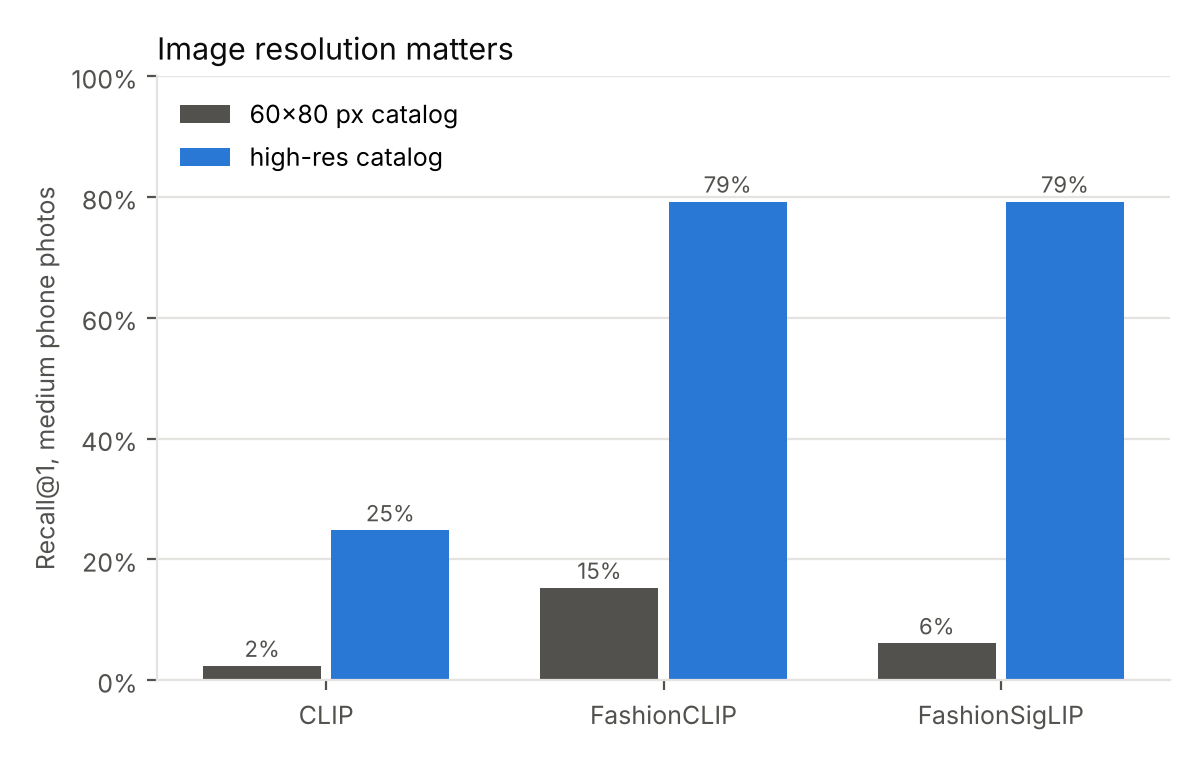
\includegraphics[width=0.62\linewidth]{fig4_resolution.png}
\caption{Effect of image resolution.}
\end{figure}

\subsection{The results ladder}\label{sec:ladder}

\begin{table}[H]
\centering
\small
\begin{tabular}{llccccccr}
\toprule
& & \multicolumn{3}{c}{Recall@1 (\%)} & R@5 (\%) & \multicolumn{2}{c}{P@5} & latency \\
\cmidrule(lr){3-5}\cmidrule(lr){7-8}
row & method & mild & medium & strong & medium & clean & medium & (ms) \\
\midrule
--  & random                     & 0.0  & 0.0  & 0.0  & 0.0  & 0.07 & 0.08 & 0.01 \\
0   & colour histogram           & 2.4  & 1.0  & 0.3  & 2.7  & 0.32 & 0.08 & 4 \\
0c  & colour histogram + crop    & 5.8  & 2.4  & 1.0  & 7.1  & 0.16 & 0.13 & 232 \\
1   & CLIP ViT-B/32              & 53.1 & 24.8 & 10.2 & 44.2 & 0.85 & 0.58 & 11 \\
2   & FashionSigLIP              & 94.9 & 79.3 & 51.0 & 91.2 & 0.90 & 0.89 & 18 \\
2b  & FashionCLIP                & 91.8 & 79.3 & 49.7 & 89.8 & 0.90 & 0.85 & 18 \\
3   & SigLIP + crop (query)      & 93.2 & 73.8 & 44.2 & 86.1 & 0.89 & 0.86 & 252 \\
3b  & SigLIP + crop (both)       & 93.9 & 74.5 & 39.1 & 86.1 & 0.90 & 0.86 & 253 \\
3c  & FashionCLIP + crop (query) & 89.5 & 71.1 & 42.2 & 84.7 & 0.90 & 0.85 & 266 \\
4   & SigLIP + multi-view        & 96.9 & 82.3 & 54.4 & 92.2 & 0.90 & 0.89 & 19 \\
4b  & FashionCLIP + multi-view   & 94.9 & 81.6 & 54.1 & 94.2 & 0.89 & 0.86 & 18 \\
5   & ensemble                   & 95.6 & 84.0 & 55.8 & 92.9 & 0.90 & 0.88 & 37 \\
5b  & ensemble, multi-view       & 96.3 & 85.4 & 58.2 & 94.9 & 0.90 & 0.88 & 37 \\
7   & fine-tuned SigLIP          & \textbf{99.0} & \textbf{96.9} & \textbf{84.7} & \textbf{99.3} & 0.81 & 0.80 & 14 \\
\bottomrule
\end{tabular}
\caption{All methods on the 294 test queries. P@5 = same-article-type Precision@5 (chance 0.07).
Selected 95\% CIs (Recall@1): FashionSigLIP medium [74, 84], strong [45, 56];
ensemble multi-view medium [81, 89], strong [52, 64]; fine-tuned medium [95, 99], strong [80, 89].
Latency was measured on the laptop GPU while other jobs sometimes ran, so small differences
(e.g.\ 14 vs 18 ms for two models of identical size) are noise.}
\label{tab:ladder}
\end{table}

\begin{figure}[H]
\centering
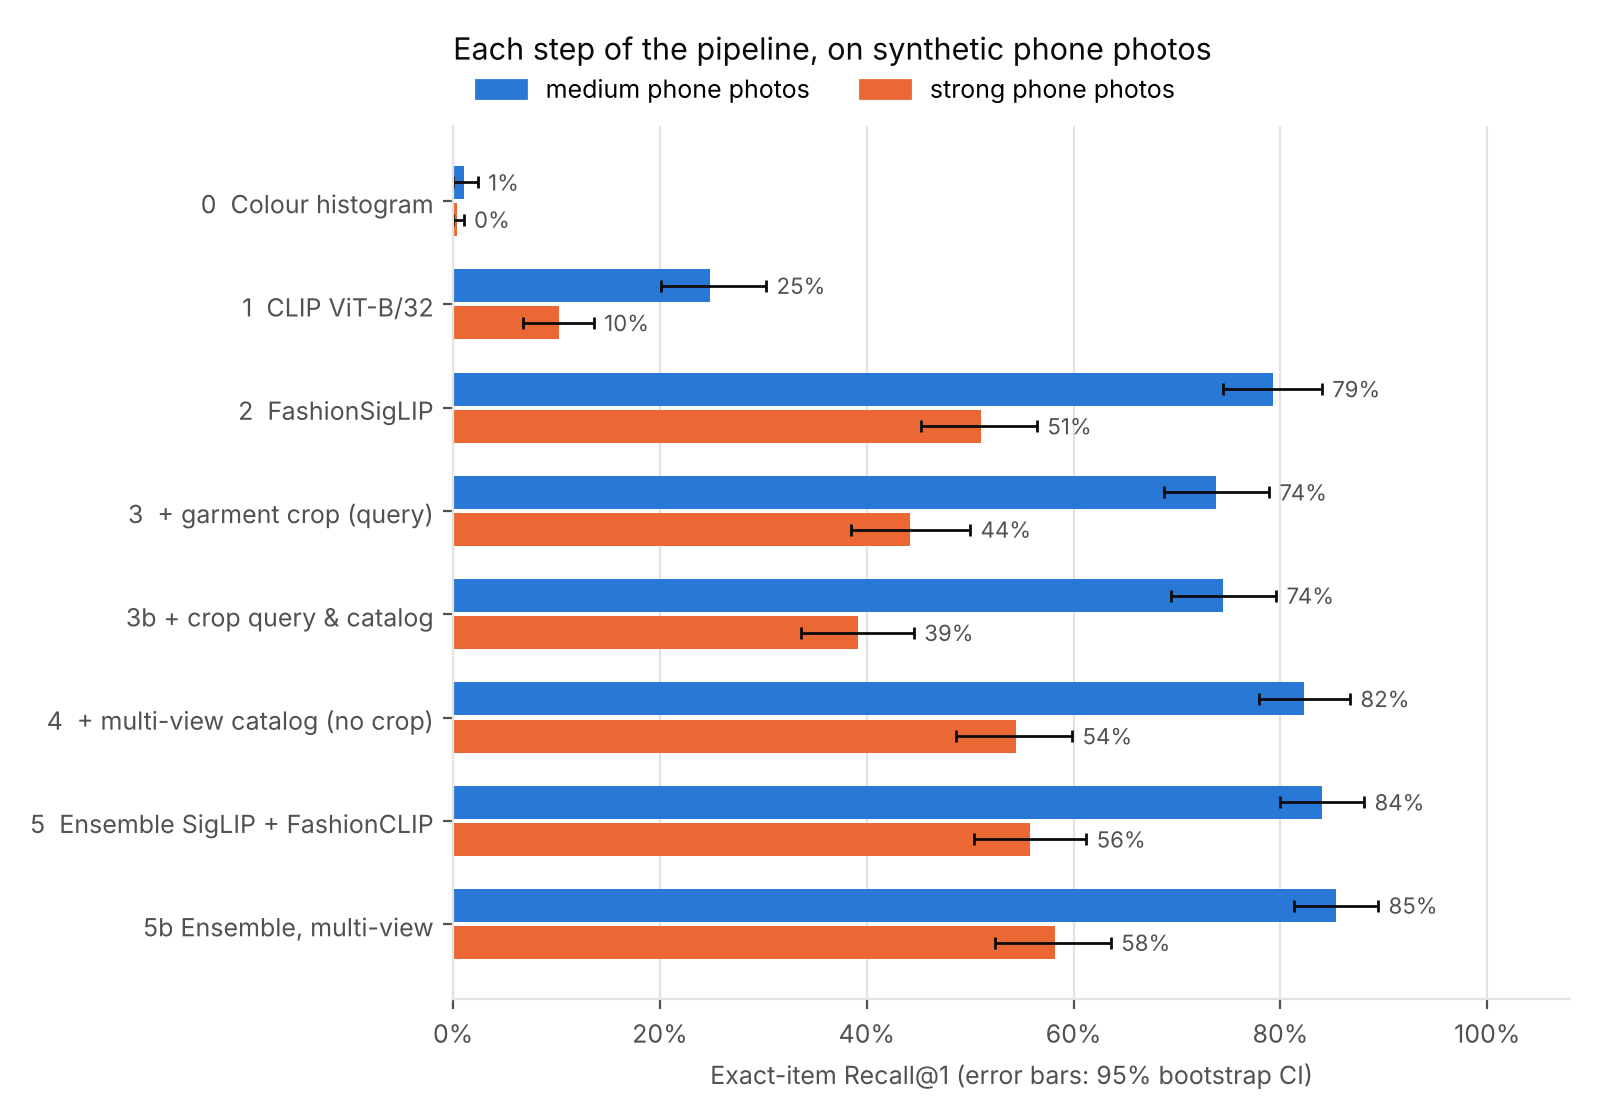
\includegraphics[width=0.75\linewidth]{fig1_ladder.png}
\caption{Results ladder (Recall@1 on phone photos).}
\end{figure}

\subsection{Which differences are real}

\begin{table}[H]
\centering
\small
\begin{tabular}{lccc}
\toprule
change (Recall@1) & mild & medium & strong \\
\midrule
colour histogram $\to$ CLIP       & +50.7* & +23.8* & +9.9* \\
CLIP $\to$ FashionCLIP            & +38.8* & +54.4* & +39.5* \\
FashionCLIP $\to$ FashionSigLIP   & +3.1 ($p$=0.06) & +0.0 ($p$=1.0) & +1.4 ($p$=0.61) \\
SigLIP $\to$ + crop (query)       & $-$1.7 ($p$=0.25) & $-$5.4* & $-$6.8* \\
SigLIP $\to$ + crop (both)        & $-$1.0 ($p$=0.54) & $-$4.8* ($p$=0.04) & $-$11.9* \\
SigLIP $\to$ + multi-view         & +2.0* & +3.1* & +3.4* \\
SigLIP $\to$ ensemble             & +0.7 ($p$=0.64) & +4.8* & +4.8* \\
ensemble $\to$ ensemble multi-view & +0.7 ($p$=0.48) & +1.4 ($p$=0.11) & +2.4* ($p$=0.035) \\
SigLIP $\to$ fine-tuned           & +4.1* & +17.7* & +33.7* \\
\midrule
change (Precision@5) & & & \\
SigLIP $\to$ fine-tuned           & $-$10.3* & $-$8.8* & $-$2.9* ($p$=0.047) \\
\bottomrule
\end{tabular}
\caption{Paired bootstrap differences in percentage points. * = significant at 0.05.
Where no $p$ is shown, $p<0.03$; for the fine-tuning rows and the large early steps, $p<0.0005$.
Full table with CIs: \texttt{results/comparisons.csv}.}
\end{table}

\paragraph{Interpretation.}
\begin{itemize}
  \item \textbf{Fashion-specific pretraining is the biggest single gain} (+39 to +54 points over CLIP).
        CLIP was trained on general internet images; the fashion models were trained on product
        photos, which is exactly our catalogue.
  \item \textbf{The two fashion models are tied.} No significant difference at any severity. We use
        FashionSigLIP as the base for fine-tuning because it is marginally ahead on strong photos and
        Precision@5, not because it is proven better.
  \item \textbf{Multi-view catalogue embeddings: small, consistent, free.} +2--3 points, significant at
        all severities, with no extra cost at search time (the extra work is done once, offline).
  \item \textbf{The ensemble helps on harder photos} (+4.8 points on medium and strong, no difference on
        mild), which suggests the two models make different mistakes. It doubles search time (37 vs
        18 ms).
  \item \textbf{Garment cropping significantly hurts}, and cropping the catalogue too does not fix it,
        so the cause is not a framing mismatch between query and catalogue. The likely cause is that
        rembg's segmentation fails on our synthetic backgrounds (not yet inspected). Our synthetic photos
        contain no person or room, which is what cropping is meant to remove, so this test cannot show
        cropping's intended benefit. It also costs about 230 ms per query, about 12$\times$ the
        embedding time. For the colour histogram, cropping helps slightly (R@1 1.0 $\to$ 2.4\% on medium,
        P@5 0.08 $\to$ 0.13), as expected: without cropping, the histogram is dominated by the background.
  \item \textbf{Mild photos are nearly solved} (95--97\% before fine-tuning); medium and strong are
        where methods separate.
\end{itemize}

\subsection{Robustness and cost}

\begin{figure}[H]
\centering
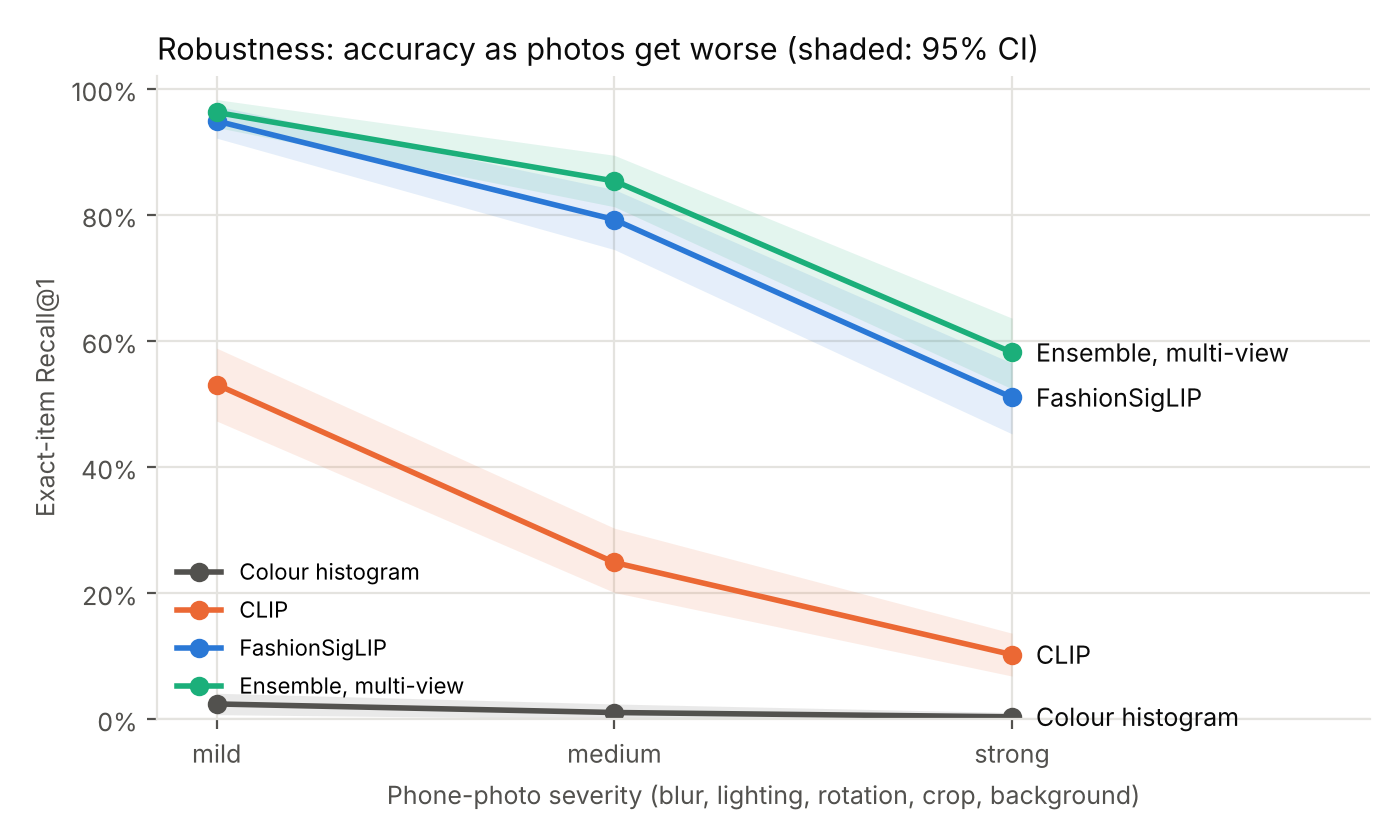
\includegraphics[width=0.75\linewidth]{fig2_robustness.png}
\caption{Recall@1 against photo severity. All methods degrade; the fashion models degrade far more
gracefully than CLIP.}
\end{figure}

\begin{figure}[H]
\centering
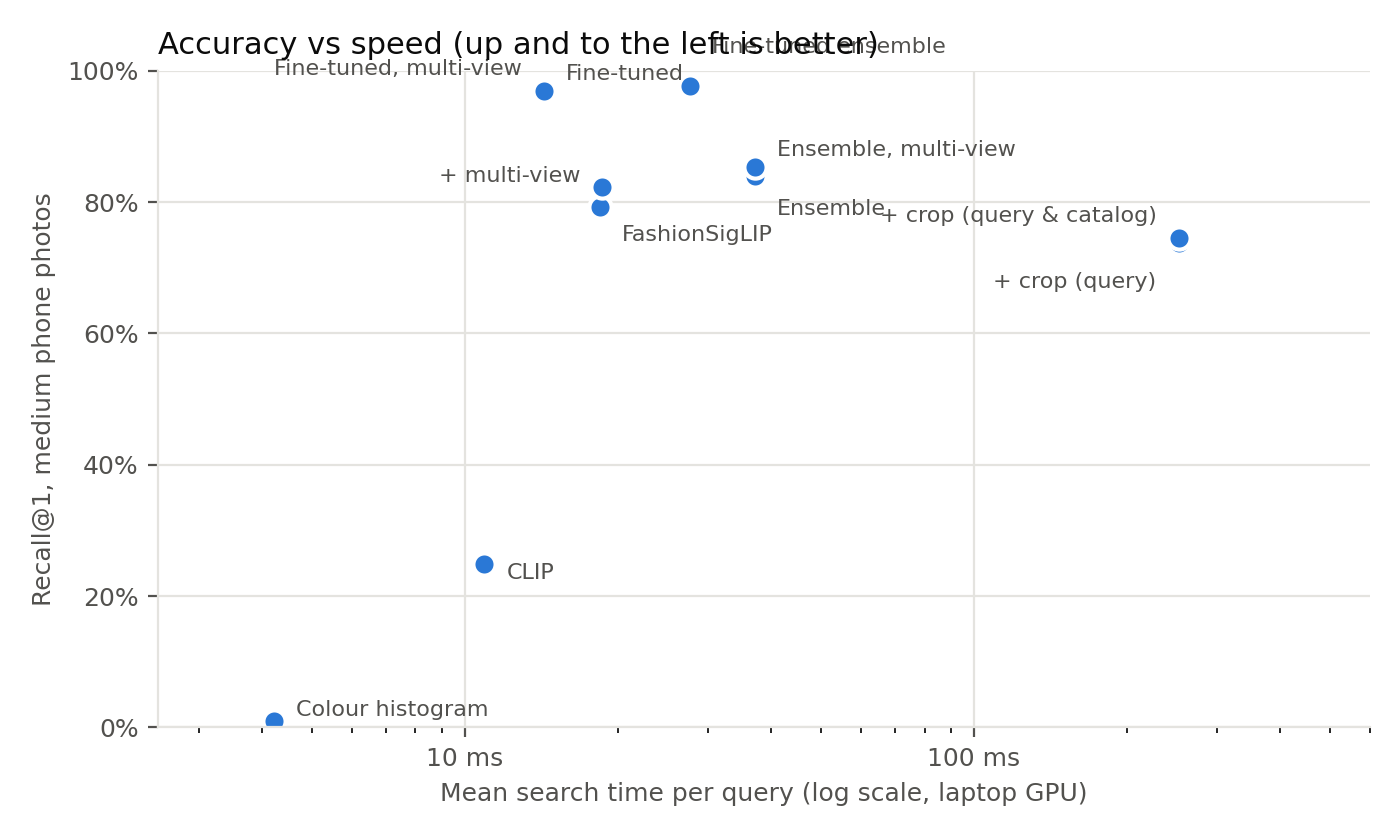
\includegraphics[width=0.75\linewidth]{fig3_tradeoff.png}
\caption{Accuracy vs search latency. Cropping is both slower and worse; the ensemble buys about
5 points for 2$\times$ latency.}
\end{figure}

\clearpage
%=====================================================================
\section{Fine-tuning}\label{sec:ft}

\subsection{Setup}
\begin{itemize}
  \item \textbf{Training pairs}: for each of the 5,603 training items (catalogue minus test items minus
        validation items), a fresh synthetic phone photo (random severity, new random draws every epoch)
        paired with its clean shop photo.
  \item \textbf{Loss}: contrastive with in-batch negatives. A batch of $B=64$ pairs gives a
        $64\times64$ matrix of cosine similarities (divided by a temperature of 0.05). For phone photo $i$,
        the right answer is shop photo $i$ and the other 63 are wrong; cross-entropy in both directions
        (phone$\to$shop and shop$\to$phone), averaged.
  \item \textbf{Hard batches}: every batch contains items of the \emph{same} article type, so the
        negatives are similar garments (other T-shirts, not shoes).
  \item \textbf{Size}: only the last 4 of 12 transformer blocks (plus the final pooling/projection
        layers) are trained: 35.4M of the encoder's 92.9M parameters. Learning rate $10^{-5}$,
        5 epochs, about 26 minutes on the laptop GPU.
  \item \textbf{Validation}: 300 held-out non-test items, one fixed medium phone photo each, searched
        against the 5,903-image gallery (catalogue minus test items). The best epoch is kept.
\end{itemize}

\subsection{Training curve}

\begin{table}[H]
\centering
\begin{tabular}{cccc}
\toprule
epoch & train loss & val Recall@1 & val Recall@5 \\
\midrule
0 (pretrained) & --    & 0.807 & -- \\
1 & 0.501 & 0.957 & 0.997 \\
2 & 0.162 & 0.973 & 0.997 \\
3 & 0.114 & \textbf{0.977} (saved) & 0.997 \\
4 & 0.091 & 0.977 & 1.000 \\
5 & 0.091 & 0.977 & 1.000 \\
\bottomrule
\end{tabular}
\caption{Fine-tuning log (\texttt{models/finetune\_log.csv}).}
\end{table}

Almost all of the gain comes in the first epoch (+15 points); the curve plateaus after epoch 3.
The validation set is close to its ceiling (Recall@5 $\approx$ 100\%), so it can no longer separate
epochs. Sanity check: the pretrained model scores 80.7\% on validation and 79.3\% on the medium test
queries, so the validation setup behaves like the test setup.

\subsection{Test results and the trade-off}

On the 294 test queries, fine-tuning raises Recall@1 significantly at every severity, and the gain grows
with difficulty: +4.1 (mild), +17.7 (medium), +33.7 points (strong; 51.0\% $\to$ 84.7\%).
Recall@5 on strong photos goes from 65.6\% to 95.6\%.

However, \textbf{same-type Precision@5 drops significantly}: $-10.3$ (mild), $-8.8$ (medium) and a
small, borderline $-2.9$ points (strong, $p=0.047$; it would not survive a Bonferroni correction over
the six tests). The clean-query P@5 drops from 0.90 to 0.81.

\paragraph{Likely explanation (hypothesis).} With same-type hard batches, every negative is the same
article type as the positive. The loss therefore explicitly pushes \emph{this} T-shirt away from all
the \emph{other} T-shirts. The model becomes very good at separating the exact item from lookalikes,
but loses the property that T-shirts sit near T-shirts, so ranks 2--5 fill with items of other types.
This is testable: retrain with random batches (\texttt{--hard\_batches 0}) and see whether P@5
recovers. \pending{ablation.}

\paragraph{Why this matters for the stakeholder.} If the exact item is out of stock, the shop wants
to offer similar items. Fine-tuning trades that ability for exact-match accuracy.

%=====================================================================
\section{Real photos: LookBench}\label{sec:lookbench}

The fine-tuning caveat is that training and validation use the same synthetic augmentation as the test
set, so part of the gain may be ``learning the augmentation''. Only real photos can check this.
LookBench (Gao et al., 2026) is an open fashion-retrieval benchmark; we use its \texttt{real\_streetlook}
subset: 981 real street-style photos as queries against a 3,278-image product gallery. As in
LookBench's own evaluation code, a result is correct if it has the same item ID as the query. Queries
are LookBench's own garment crops (\texttt{--query\_image image}).

\begin{table}[H]
\centering
\begin{tabular}{lccc}
\toprule
method & Recall@1 (\%) & Recall@5 (\%) & Category P@5 \\
\midrule
FashionSigLIP & 42.8 [39.8, 45.8] & 64.1 [61.3, 67.0] & 0.714 [0.692, 0.736] \\
fine-tuned    & 45.5 [42.6, 48.4] & 67.3 [64.4, 70.2] & 0.691 [0.670, 0.712] \\
\midrule
paired difference & +2.7 [+0.5, +4.8]* & +3.2 & $-$0.023 [$-$0.034, $-$0.012]* \\
\bottomrule
\end{tabular}
\caption{LookBench \texttt{real\_streetlook}, 981 queries, 95\% bootstrap CIs.
* = significant in a paired bootstrap ($p=0.014$ for Recall@1, $p<0.0005$ for category P@5).}
\end{table}

\paragraph{Interpretation.}
\begin{itemize}
  \item \textbf{The fine-tuning gain shrinks from +17.7 points (synthetic medium) to about +2.7
        points (real).} Most of the synthetic gain was the model learning our augmentation, not getting
        better at real phone photos. This confirms the caveat with evidence.
  \item The small gain is real: the paired bootstrap gives +2.7 points [+0.5, +4.8], $p=0.014$.
        Note that the two separate CIs overlap, yet the paired test is significant: because both models
        answer the same 981 queries, query difficulty cancels out in the differences.
  \item The category trade-off appears on real data too ($-$2.3 points category P@5, $p<0.0005$),
        so it is not only a property of the synthetic photos.
  \item Absolute numbers are much lower on real photos (43\% vs 79\% Recall@1 for FashionSigLIP),
        so our synthetic phone photos are \emph{easier} than reality. This is a limitation of the
        synthetic test set and must be stated.
\end{itemize}
\paragraph{Comparison with the LookBench paper.} Our numbers are \emph{not} directly comparable with
the paper's. The paper's headline metric is \emph{fine Recall@1}: the top result must have the query's
category and all of its annotated attributes, searched against a 61,553-image corpus (positives plus
Fashion200K distractors). We use the public release (3,278 gallery images, no distractors) and count a
result as correct only if it has the same \texttt{item\_ID}. The paper reports, for FashionSigLIP on
RealStreetLook, fine Recall@1 55.2\%, coarse (category-only) Recall@1 73.4\% and nDCG@5 42.4. The closest
comparable quantity we have is category Precision@5 = 71.4\%, which is consistent with their 73.4\%
(not the same metric: ours averages over the top 5). The gap between our 42.8\% and their 55.2\% is
therefore a difference in definition (smaller gallery vs.\ a different notion of ``correct''), not
evidence of a scoring bug. \pending{optional: also record category Recall@1, which is exactly the
paper's coarse Recall@1, for a direct check.}

%=====================================================================
\section{Conformal retrieval}\label{sec:conformal}

\paragraph{Idea.} Instead of always returning 5 items, return a \emph{set} that contains the true item
with probability at least $1-\alpha$ (e.g.\ 90\%). A staff member then only checks this shortlist:
small sets when the model is sure, larger sets when it is not.

\paragraph{Method (split conformal).} Split the labelled phone queries at random into a calibration
half and a test half.
\begin{itemize}
  \item \emph{Threshold variant}: on the calibration half let $s_i$ = similarity between query $i$
        and its true item. Choose $\tau$ = the $k$-th smallest $s_i$ with
        $k=\lfloor (n+1)\alpha \rfloor$. For a new query, return every item with similarity
        $\ge \tau$.
  \item \emph{Relative variant}: let $r_i$ = (best similarity of query $i$) $-$ (similarity to its true
        item) $\ge 0$. Choose $q$ = the $k$-th smallest $r_i$ with $k=\lceil (n+1)(1-\alpha)\rceil$.
        Return every item within $q$ of the query's best similarity. Easy queries (clear winner) get
        small sets.
\end{itemize}

\paragraph{Guarantee.} If calibration and test queries are exchangeable (drawn the same way), then for a
new query $P(\text{true item} \in \text{set}) \ge 1-\alpha$. Sketch: the new query's score is equally
likely to land in any of the $n+1$ positions when sorted with the $n$ calibration scores, so it falls
beyond the $k$-th one with probability at most $\alpha$. No assumption about the model or the data
distribution is needed, only exchangeability.

\paragraph{Status.} The code (\texttt{evaluation/conformal.py}) has unit tests and was validated on
simulated scores: coverage hit the target; the relative variant gave sets about 30\% smaller; and
deliberately breaking exchangeability (calibrating on mild photos, testing on strong ones) dropped
90\% target coverage to about 63\%. That last result is the point of the shift experiment: the
guarantee holds only when calibration data looks like deployment data.
\pending{run on real models: \texttt{ensemble\_mv}, \texttt{fashion\_siglip}, and now the fine-tuned
model; add a coverage / set-size figure.}

%=====================================================================
\section{Summary of findings so far}

\begin{enumerate}
  \item High-resolution images were essential (6\% $\to$ 79\% Recall@1 for FashionSigLIP).
  \item Learned embeddings vastly beat the colour histogram (1\% $\to$ 79\% on medium photos).
  \item Domain-specific pretraining is the largest gain; the two fashion models are tied.
  \item Multi-view (+2--3, free) and the ensemble (+5, 2$\times$ latency) give significant extra gains.
  \item rembg garment cropping significantly hurts on synthetic photos and is 12$\times$ slower.
  \item Fine-tuning gives a large synthetic gain (+18 to +34 points) but only +2.7 on real photos
        (still significant, $p=0.014$), and costs same-type Precision@5 (about $-$9 points synthetic,
        $-$2.3 real).
  \item Synthetic phone photos are easier than real street photos (79\% vs 43\%).
\end{enumerate}

\section{Limitations}
\begin{itemize}
  \item The main test set is synthetic; real-photo results so far are LookBench only. Own photos of
        real garments are pending.
  \item 294 test queries is small; every number carries a CI, but small differences ($<$3 points) are
        hard to establish.
  \item Fine-tuning trains on the same augmentation family it is tested on (shown by LookBench).
  \item Latency so far is measured on a laptop GPU, not on the CPU a deployed service would use.
  \item Our LookBench metric (same \texttt{item\_ID}, small gallery) differs from the paper's fine
        Recall@1, so our real-photo numbers cannot be placed on the paper's leaderboard.
\end{itemize}

\section{Remaining work}
\begin{enumerate}
  \item Problem framing: confirm stakeholder and real-world constraint from the approved proposal.
  \item ``How it's done today'' baseline: filter by category + colour using catalogue labels.
  \item Evaluate \texttt{finetuned\_mv} and \texttt{ensemble\_ft\_mv} (synthetic and LookBench).
  \item Conformal retrieval on real models, with figure; fine-tuning curve figure.
  \item About 30 own photos (Precision@5).
  \item Production: FastAPI \texttt{/search} (uploads kept in memory only), Streamlit UI, Docker,
        CPU latency in Docker.
  \item Analysis: failure gallery, per-category breakdown, rembg failure inspection, manual check of
        about 30 queries.
  \item Responsible ML with evidence: human oversight, robustness/shift, privacy, fairness.
  \item README, final report, poster, talk, mock Q\&A.
\end{enumerate}

\appendix
\section{Reproducing the results}
Run from the repository root with the virtual environment active.
\begin{verbatim}
export PYTORCH_ENABLE_MPS_FALLBACK=1
python -m data_prep.build_catalog
python -m data_prep.hires_catalog \
    --zip data/raw_full/fashion-product-images-dataset.zip
python -m data_prep.make_queries
python -m evaluation.run_eval --method fashion_siglip
python -m evaluation.compare fashion_siglip finetuned
python -m evaluation.compare fashion_siglip finetuned --metric p5
python -m training.finetune
python -m evaluation.run_lookbench --subset real_streetlook \
    --method finetuned
python -m report.make_figures
\end{verbatim}
Raw results: \texttt{results/summary.csv} (all metrics + CIs), \texttt{results/comparisons.csv}
(paired tests), \texttt{results/lookbench\_summary.csv}, \texttt{models/finetune\_log.csv}.

\end{document}
